\documentclass[a4paper]{article}
\input{tex/lib/barrel.tex}

\begin{document}

\include{tex/pages/титульник}

\tableofcontents
\newpage

\section*{Введение}
\addcontentsline{toc}{section}{Введение}

Код Грея~--- способ кодирования последовательных чисел, при котором соседние значения отличаются ровно в одном бите. Это свойство минимизирует ошибки при переходе между состояниями и применяется в цифровой электронике, системах передачи данных и адресации.

Мультимножества обобщают классические множества, допуская повторение элементов с заданной кратностью. Они используются в базах данных, статистике и комбинаторике.

В данной работе реализована программа генерации бинарного кода Грея для заполнения универсума мультимножеств, а также выполнения теоретико-множественных и арифметических операций над ними.

\section{Постановка задачи}

В рамках курсовой работы необходимо реализовать калькулятор <<большой>> конечной арифметики $\langle Z_i; +, * \rangle$ (8 разрядов) для четырёх действий ($+$, $-$, $*$, $/$) на основе <<малой>> конечной арифметики, где задано правило <<$+1$>> и выполняются свойства коммутативности ($+$, $*$), ассоциативности ($+$, $*$), дистрибутивности $*$ относительно $+$, заданы аддитивная единица <<$a$>> и мультипликативная единица <<$b$>>, а также выполняется свойство: $(\forall x) \; x * a = a$.

Необходимо реализовать программу, которая:

\begin{itemize}
    \item поддерживает все четыре действия, а именно:
    \begin{itemize}
        \item сложение,
        \item вычитание,
        \item умножение,
        \item деление, в т.ч. с остатком;
    \end{itemize}
    
    \item поддерживает числа до 8 разрядов включительно (например, возможно выражение $bbb + ccc$);
    
    \item поддерживает отрицательные числа;
    
    \item выполняет вычисления только в рамках данной арифметики без перевода в иные системы счисления.
\end{itemize}

\section{Математическое описание}

\subsection{Булева функция и её таблица истинности.}

Функции $f: E_2^n \to E_2$, где $E_2 = \{0, 1\}$, называются функциями алгебры логики, или булевыми функциями от $n$ переменных, по имени Дж.~Буля.

В данной работе рассматривается функция $f(x_1, x_2, x_3, x_4)$ четырёх переменных, заданная вектором значений. Функция задана десятичным числом 11011, которое в двоичной системе счисления (с заполнением первых разрядом нулями, пока не достигнем 16 разрядов) имеет вид:
\[
11011_{10} = 0010101100000011_2.
\]

Таблица истинности~--- это способ задания булевой функции, в котором для каждого из $2^n$ наборов значений переменных указано значение функции. Таблица истинности для заданной булевой функции представлена в таблице~\ref{tab:truth-table}.

\begin{table}[H]
\centering
\begin{tabular}{|c|c|c|c|c|c|}
\hline
№ & $x_1$ & $x_2$ & $x_3$ & $x_4$ & $f$ \\
\hline
0  & 0 & 0 & 0 & 0 & 0 \\
1  & 0 & 0 & 0 & 1 & 0 \\
2  & 0 & 0 & 1 & 0 & 1 \\
3  & 0 & 0 & 1 & 1 & 0 \\
4  & 0 & 1 & 0 & 0 & 1 \\
5  & 0 & 1 & 0 & 1 & 0 \\
6  & 0 & 1 & 1 & 0 & 1 \\
7  & 0 & 1 & 1 & 1 & 1 \\
8  & 1 & 0 & 0 & 0 & 0 \\
9  & 1 & 0 & 0 & 1 & 0 \\
10 & 1 & 0 & 1 & 0 & 0 \\
11 & 1 & 0 & 1 & 1 & 0 \\
12 & 1 & 1 & 0 & 0 & 0 \\
13 & 1 & 1 & 0 & 1 & 0 \\
14 & 1 & 1 & 1 & 0 & 1 \\
15 & 1 & 1 & 1 & 1 & 1 \\
\hline
\end{tabular}
\caption{Таблица истинности функции $f(x_1, x_2, x_3, x_4)$}
\label{tab:truth-table}
\end{table}

\subsection{Совершенная дизъюнктивная нормальная форма.}

Булева функция $f(x_1, \ldots, x_n)$ представима в виде формулы:
\[
\bigvee_{\{(\sigma_1,\ldots,\sigma_n) \mid f(\sigma_1,\ldots,\sigma_n)=1\}} x_1^{\sigma_1} \land \ldots \land x_n^{\sigma_n}.
\]
Такая запись называется совершенной дизъюнктивной нормальной формой (СДНФ). Всякая булева функция имеет единственную СДНФ.

Для заданной функции:
\begin{multline*}
\text{СДНФ } f = \overline{x_1}\,\overline{x_2}\,x_3\,\overline{x_4} \lor \overline{x_1}\,x_2\,\overline{x_3}\,\overline{x_4} \lor \overline{x_1}\,x_2\,x_3\,\overline{x_4} \lor \overline{x_1}\,x_2\,x_3\,x_4 \lor {} \\
{}  \lor x_1\,x_2\,x_3\,\overline{x_4} \lor x_1\,x_2\,x_3\,x_4
\end{multline*}

\subsection{Совершенная конъюнктивная нормальная форма.}

Булева функция $f(x_1, \ldots, x_n)$ представима в виде формулы:
\[
\bigwedge_{\{(\sigma_1,\ldots,\sigma_n) \mid f(\sigma_1,\ldots,\sigma_n)=0\}} (x_1^{\overline{\sigma_1}} \lor \ldots \lor x_n^{\overline{\sigma_n}}).
\]
Такая запись называется совершенной конъюнктивной нормальной формой (СКНФ). Всякая булева функция имеет единственную СКНФ.

Для заданной функции (f=0 на наборах 0, 1, 3, 5, 8, 9, 10, 11, 12, 13):
\begin{multline*}
\text{СКНФ } f = (x_1 \lor x_2 \lor x_3 \lor x_4) \land (x_1 \lor x_2 \lor x_3 \lor \overline{x_4}) \land (x_1 \lor x_2 \lor \overline{x_3} \lor \overline{x_4}) \land {} \\
{} \land (x_1 \lor \overline{x_2} \lor x_3 \lor \overline{x_4}) \land (\overline{x_1} \lor x_2 \lor x_3 \lor x_4) \land (\overline{x_1} \lor x_2 \lor x_3 \lor \overline{x_4}) \land {} \\
{} \land (\overline{x_1} \lor x_2 \lor \overline{x_3} \lor x_4) \land (\overline{x_1} \lor x_2 \lor \overline{x_3} \lor \overline{x_4}) \land (\overline{x_1} \lor \overline{x_2} \lor x_3 \lor x_4) \land {} \\
{} \land (\overline{x_1} \lor \overline{x_2} \lor x_3 \lor \overline{x_4})
\end{multline*}

\subsection{Полином Жегалкина.}

Полином Жегалкина~--- представление булевой функции в базисе $\{\land, \oplus, 1\}$, где $\oplus$~--- сложение по модулю 2.

Полином Жегалкина имеет вид:
\[
f(x_1, \ldots, x_n) = a_0 \oplus \bigoplus_{i} a_i x_i \oplus \bigoplus_{i<j} a_{ij} x_i x_j \oplus \ldots \oplus a_{12\ldots n} x_1 x_2 \ldots x_n.
\]

Для заданной функции полином Жегалкина, вычисленный методом треугольника:
\[
f = x_3 \oplus x_3 x_4 \oplus x_2 \oplus x_2 x_4 \oplus x_2 x_3 \oplus x_1 x_3 \oplus x_1 x_3 x_4 \oplus x_1 x_2 \oplus x_1 x_2 x_4.
\]

\subsection{Выбор порядка переменных.} 

Порядок следования переменных выбирается с целью получения наиболее компактной бинарной диаграммы решений.

Производная показывает, на каких наборах значение функции меняется при изменении $x_i$. Чем больше единиц в таблице истинности производной, тем сильнее функция зависит от переменной.

Количество единиц в таблице истинности производных (см. раздел <<производные булевой функции>>):
\begin{itemize}
    \item $\dfrac{\partial f}{\partial x_1}$: 2 единицы~--- функция слабо зависит от $x_1$
    \item $\dfrac{\partial f}{\partial x_2}$: 4 единицы~--- функция сильно зависит от $x_2$
    \item $\dfrac{\partial f}{\partial x_3}$: 4 единицы~--- функция сильно зависит от $x_3$
    \item $\dfrac{\partial f}{\partial x_4}$: 2 единицы~--- функция слабо зависит от $x_4$
\end{itemize}

Для построения компактной БДР важно не только количество единиц в производных, но и возможность объединения эквивалентных поддеревьев. Проанализируем поведение функции при фиксации переменных.

Для упрощения оценки рассмотрим ДНФ, мининизированную с помощью алгеброических преобразований: 

\begin{align*}
f &= \overline{x_1}\,\overline{x_2}\,x_3\,\overline{x_4} \lor \overline{x_1}\,x_2\,\overline{x_3}\,\overline{x_4} \lor \overline{x_1}\,x_2\,x_3\,\overline{x_4} \lor \overline{x_1}\,x_2\,x_3\,x_4 \lor x_1\,x_2\,x_3\,\overline{x_4} \lor x_1\,x_2\,x_3\,x_4 \\
&= \overline{x_1}\,\overline{x_2}\,x_3\,\overline{x_4} \lor \overline{x_1}\,x_2\,\overline{x_3}\,\overline{x_4} \lor \overline{x_1}\,x_2\,x_3 \lor x_1\,x_2\,x_3 \\
&= \overline{x_1}\,\overline{x_2}\,x_3\,\overline{x_4} \lor \overline{x_1}\,x_2\,\overline{x_3}\,\overline{x_4} \lor x_2\,x_3 \\
\end{align*}

\begin{itemize}
    \item При $x_1 = 1$: первые два терма обнуляются, и функция упрощается до $f = x_2\,x_3$. Это означает, что при $x_1 = 1$ всё поддерево заменяется простой функцией двух переменных.
    
    \item При $x_1 = 1$ значение функции не зависит от $x_4$, что позволяет пропустить проверку $x_4$ в этой ветви.
    
    \item При $x_1 = 0$ и $x_4 = 1$: функция также упрощается до $f = x_2\,x_3$. Поддеревья при $(x_1 = 1)$ и $(x_1 = 0, x_4 = 1)$ эквивалентны и могут быть объединены в БДР.
\end{itemize}

Таким образом, если поставить $x_1$ первой переменной, а $x_4$ второй, то:
\begin{itemize}
    \item при $x_1 = 1$ можно полностью исключить проверку $x_4$;
    \item поддеревья для $(x_1 = 1)$ и $(x_1 = 0, x_4 = 1)$ совпадают и объединяются.
\end{itemize}

Выбираем порядок переменных: $x_1, x_4, x_2, x_3$.

\subsection{Семантическое дерево.} 

Таблицу истинности булевой функции $n$ переменных можно представить в виде бинарного дерева высоты $n+1$. Ярусы дерева соответствуют переменным, дуги~--- значениям переменных (пунктирная линия~--- 0, сплошная~--- 1).

Семантическое дерево для заданной функции с порядком переменных $x_1, x_4, x_2, x_3$ представлено на рис.~\ref{fig:semantic-tree}.

\begin{figure}[H]
\centering
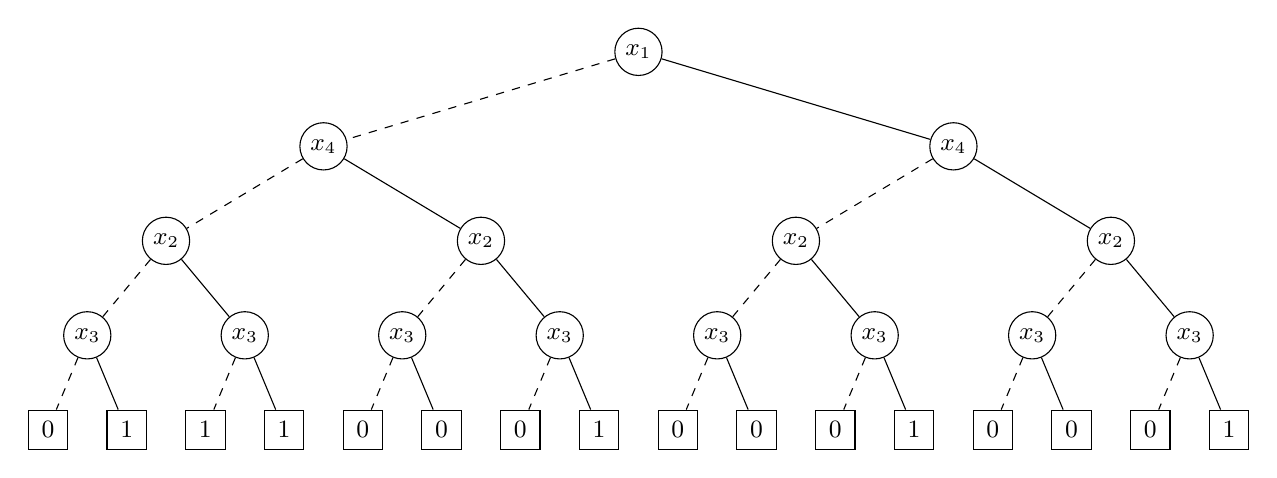
\begin{tikzpicture}[
    level 1/.style={sibling distance=80mm, level distance=12mm},
    level 2/.style={sibling distance=40mm, level distance=12mm},
    level 3/.style={sibling distance=20mm, level distance=12mm},
    level 4/.style={sibling distance=10mm, level distance=12mm},
    every node/.style={circle, draw, solid, minimum size=6mm, inner sep=1pt, font=\small},
    leaf/.style={rectangle, draw, solid, minimum size=5mm, inner sep=2pt, font=\small},
    edge0/.style={dashed},
    edge1/.style={solid}
]
\node {$x_1$}
    child {node {$x_4$}
        child {node {$x_2$}
            child {node {$x_3$}
                child {node[leaf] {0} edge from parent[edge0]}
                child {node[leaf] {1} edge from parent[edge1]}
                edge from parent[edge0]
            }
            child {node {$x_3$}
                child {node[leaf] {1} edge from parent[edge0]}
                child {node[leaf] {1} edge from parent[edge1]}
                edge from parent[edge1]
            }
            edge from parent[edge0]
        }
        child {node {$x_2$}
            child {node {$x_3$}
                child {node[leaf] {0} edge from parent[edge0]}
                child {node[leaf] {0} edge from parent[edge1]}
                edge from parent[edge0]
            }
            child {node {$x_3$}
                child {node[leaf] {0} edge from parent[edge0]}
                child {node[leaf] {1} edge from parent[edge1]}
                edge from parent[edge1]
            }
            edge from parent[edge1]
        }
        edge from parent[edge0]
    }
    child {node {$x_4$}
        child {node {$x_2$}
            child {node {$x_3$}
                child {node[leaf] {0} edge from parent[edge0]}
                child {node[leaf] {0} edge from parent[edge1]}
                edge from parent[edge0]
            }
            child {node {$x_3$}
                child {node[leaf] {0} edge from parent[edge0]}
                child {node[leaf] {1} edge from parent[edge1]}
                edge from parent[edge1]
            }
            edge from parent[edge0]
        }
        child {node {$x_2$}
            child {node {$x_3$}
                child {node[leaf] {0} edge from parent[edge0]}
                child {node[leaf] {0} edge from parent[edge1]}
                edge from parent[edge0]
            }
            child {node {$x_3$}
                child {node[leaf] {0} edge from parent[edge0]}
                child {node[leaf] {1} edge from parent[edge1]}
                edge from parent[edge1]
            }
            edge from parent[edge1]
        }
        edge from parent[edge1]
    };
\end{tikzpicture}
\caption{Семантическое дерево функции $f$ (порядок $x_1, x_4, x_2, x_3$)}
\label{fig:semantic-tree}
\end{figure}

\subsection{Упрощённое семантическое дерево.}

Упрощённое семантическое дерево представлено на рис.~\ref{fig:simplified-tree}. При упрощении применяются следующие правила:
\begin{itemize}
    \item если оба потомка узла~--- одинаковые листья, узел заменяется этим листом;
    \item если поддеревья эквивалентны, они объединяются.
\end{itemize}

\begin{figure}[H]
\centering
\begin{tikzpicture}[
    level 1/.style={sibling distance=60mm, level distance=15mm},
    level 2/.style={sibling distance=35mm, level distance=15mm},
    level 3/.style={sibling distance=18mm, level distance=15mm},
    node/.style={circle, draw, solid, minimum size=8mm, inner sep=1pt, font=\small},
    leaf/.style={rectangle, draw, solid, minimum size=7mm, inner sep=2pt, font=\small},
    edge0/.style={dashed},
    edge1/.style={solid}
]
\node[node] {$x_1$}
    child {node[node] {$x_4$}
        child {node[node] {$x_2$}
            child {node[node] {$x_3$}
                child {node[leaf] {0} edge from parent[edge0]}
                child {node[leaf] {1} edge from parent[edge1]}
                edge from parent[edge0]
            }
            child {node[leaf] {1} edge from parent[edge1]}
            edge from parent[edge0]
        }
        child {node[node] {$x_2$}
            child {node[leaf] {0} edge from parent[edge0]}
            child {node[node] {$x_3$}
                child {node[leaf] {0} edge from parent[edge0]}
                child {node[leaf] {1} edge from parent[edge1]}
                edge from parent[edge1]
            }
            edge from parent[edge1]
        }
        edge from parent[edge0]
    }
    child {node[node] {$x_2$}
        child {node[leaf] {0} edge from parent[edge0]}
        child {node[node] {$x_3$}
            child {node[leaf] {0} edge from parent[edge0]}
            child {node[leaf] {1} edge from parent[edge1]}
            edge from parent[edge1]
        }
        edge from parent[edge1]
    };
\end{tikzpicture}
\caption{Упрощённое семантическое дерево функции $f$ (порядок $x_1, x_4, x_2, x_3$)}
\label{fig:simplified-tree}
\end{figure}

При упрощении:
\begin{itemize}
    \item При $x_1 = 1$ проверка $x_4$ пропускается, так как результат не зависит от $x_4$.
    \item Поддерево при $x_1 = 1$ совпадает с поддеревом при $(x_1 = 0, x_4 = 1)$.
    \item Узлы $x_3$ с одинаковыми потомками $(0, 1)$ объединяются.
\end{itemize}

\subsection{Бинарная диаграмма решений.}

Бинарная диаграмма решений (БДР) для заданной функции представлена на рис.~\ref{fig:bdd-graph}. В БДР, в отличие от дерева, допускается повторное использование узлов~--- эквивалентные поддеревья представляются одним подграфом.

\begin{figure}[H]
\centering
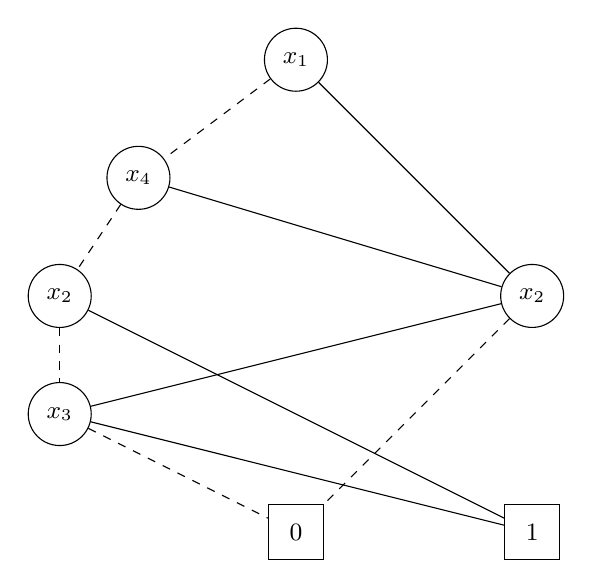
\begin{tikzpicture}[
    node/.style={circle, draw, solid, minimum size=8mm, inner sep=1pt, font=\small},
    leaf/.style={rectangle, draw, solid, minimum size=7mm, inner sep=2pt, font=\small},
    edge0/.style={dashed},
    edge1/.style={solid}
]
% Уровень 1
\node[node] (x1) at (0, 0) {$x_1$};

% Уровень 2
\node[node] (x4) at (-2, -1.5) {$x_4$};
\node[node] (x2b) at (3, -3) {$x_2$};

% Уровень 3
\node[node] (x2a) at (-3, -3) {$x_2$};

% Уровень 4
\node[node] (x3b) at (-3, -4.5) {$x_3$};

% Листья
\node[leaf] (l0) at (0, -6) {0};
\node[leaf] (l1) at (3, -6) {1};

% Рёбра от x1
\draw[edge0] (x1) -- (x4);
\draw[edge1] (x1) -- (x2b);

% Рёбра от x4
\draw[edge0] (x4) -- (x2a);
\draw[edge1] (x4) -- (x2b);

% Рёбра от x2a
\draw[edge0] (x2a) -- (x3b);
\draw[edge1] (x2a) -- (l1);

% Рёбра от x2b
\draw[edge1] (x2b) -- (x3b);
\draw[edge0] (x2b) -- (l0);

% Рёбра от x3b
\draw[edge0] (x3b) -- (l0);
\draw[edge1] (x3b) -- (l1);
\end{tikzpicture}
\caption{Бинарная диаграмма решений (пунктир~--- 0, сплошная~--- 1)}
\label{fig:bdd-graph}
\end{figure}

ДНФ из БДР: $f = \overline{x_1}\,\overline{x_2}\,x_3\,\overline{x_4} \lor \overline{x_1}\,x_2\,\overline{x_4} \lor \overline{x_1}\,x_2\,x_3\,x_4 \lor x_1\,x_2\,x_3$.

После упрощения даёт: $f = \overline{x_1}\,x_3\,\overline{x_4} \lor \overline{x_1}\,x_2\,\overline{x_4} \lor x_2\,x_3$.

\begin{itemize}
    \item Терм $\overline{x_1}\,\overline{x_2}\,x_3\,\overline{x_4} \lor \overline{x_1}\,x_2\,x_3\,x_4 = \overline{x_1}\,x_3\,\overline{x_4}$ (поглощение по $x_2$).
    \item Термы $\overline{x_1}\,x_2\,x_3\,x_4$ и $x_1\,x_2\,x_3$ объединяются: $x_2\,x_3\,(\overline{x_1}\,x_4 \lor x_1) = x_2\,x_3\,(x_1 \lor x_4)$, что после упрощения даёт $x_2\,x_3$.
\end{itemize}

Таким образом, БДР даёт сокращённую форму, которую в дальнейшем можно использовать для построения логической схемы.

\subsection{Синтаксическое дерево минимальной ДНФ.} 

Синтаксическое дерево~--- это представление формулы в виде дерева, где внутренние вершины соответствуют операциям, а листья~--- переменным или константам.

Синтаксическое дерево для минимальной ДНФ $f = \overline{x_1}\,x_3\,\overline{x_4} \lor \overline{x_1}\,x_2\,\overline{x_4} \lor x_2\,x_3$ представлено на рис.~\ref{fig:syntax-tree}.

\begin{figure}[H]
\centering
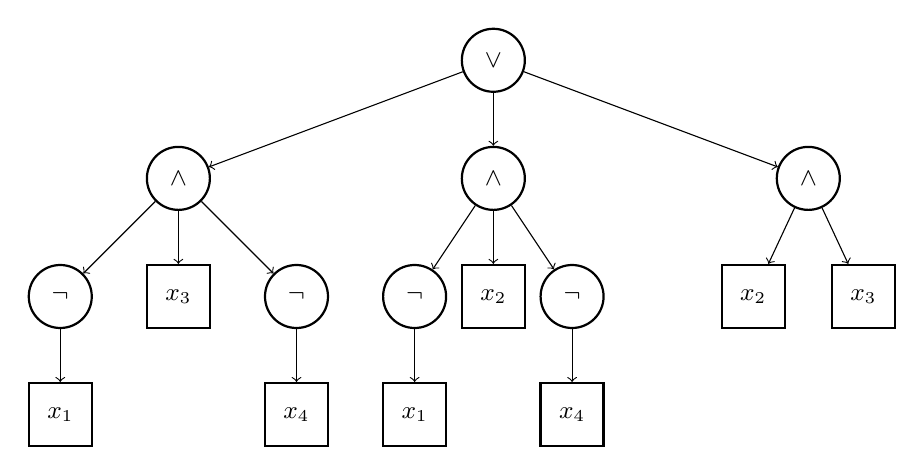
\begin{tikzpicture}[
    op/.style={circle, draw, thick, minimum size=8mm, font=\small},
    var/.style={rectangle, draw, thick, minimum size=8mm, font=\small},
]

% Уровень 0: корень
\node[op] (root) at (0, 0) {$\lor$};

% Уровень 1: три конъюнкции
\node[op] (and1) at (-4, -1.5) {$\land$};
\node[op] (and2) at (0, -1.5) {$\land$};
\node[op] (and3) at (4, -1.5) {$\land$};

% Уровень 2: операнды первой конъюнкции
\node[op] (neg1) at (-5.5, -3) {$\neg$};
\node[var] (x3a) at (-4, -3) {$x_3$};
\node[op] (neg2) at (-2.5, -3) {$\neg$};

% Уровень 2: операнды второй конъюнкции
\node[op] (neg3) at (-1, -3) {$\neg$};
\node[var] (x2a) at (0, -3) {$x_2$};
\node[op] (neg4) at (1, -3) {$\neg$};

% Уровень 2: операнды третьей конъюнкции
\node[var] (x2b) at (3.3, -3) {$x_2$};
\node[var] (x3b) at (4.7, -3) {$x_3$};

% Уровень 3: переменные под отрицаниями
\node[var] (x1a) at (-5.5, -4.5) {$x_1$};
\node[var] (x4a) at (-2.5, -4.5) {$x_4$};
\node[var] (x1b) at (-1, -4.5) {$x_1$};
\node[var] (x4b) at (1, -4.5) {$x_4$};

% Рёбра от корня
\draw[->] (root) -- (and1);
\draw[->] (root) -- (and2);
\draw[->] (root) -- (and3);

% Рёбра первой конъюнкции
\draw[->] (and1) -- (neg1);
\draw[->] (and1) -- (x3a);
\draw[->] (and1) -- (neg2);

% Рёбра второй конъюнкции
\draw[->] (and2) -- (neg3);
\draw[->] (and2) -- (x2a);
\draw[->] (and2) -- (neg4);

% Рёбра третьей конъюнкции
\draw[->] (and3) -- (x2b);
\draw[->] (and3) -- (x3b);

% Рёбра отрицаний
\draw[->] (neg1) -- (x1a);
\draw[->] (neg2) -- (x4a);
\draw[->] (neg3) -- (x1b);
\draw[->] (neg4) -- (x4b);

\end{tikzpicture}
\caption{Синтаксическое дерево минимальной ДНФ}
\label{fig:syntax-tree}
\end{figure}

\subsection{Логическая схема.}

Логическая схема~--- это схема, реализующая булеву функцию с помощью логических элементов (И, ИЛИ, НЕ).

\screenshot{image_2026-01-15_05-18-09.png}{Логическая схема для минимальной ДНФ}

\subsection{Производные булевой функции.} 

Производная булевой функции $f$ по переменной $x_i$:
\[
\frac{\partial f}{\partial x_i} = f|_{x_i = 0} \oplus f|_{x_i = 1}.
\]


Вычислим производные функции $f = \overline{x_1}\,x_3\,\overline{x_4} \lor \overline{x_1}\,x_2\,\overline{x_4} \lor x_2\,x_3$ по каждой переменной.

\subsubsection*{Производная по $x_1$.}

\[
f|_{x_1=0} = \overline{0}\,x_3\,\overline{x_4} \lor \overline{0}\,x_2\,\overline{x_4} \lor x_2\,x_3 = x_3\,\overline{x_4} \lor x_2\,\overline{x_4} \lor x_2\,x_3.
\]

\[
f|_{x_1=1} = \overline{1}\,x_3\,\overline{x_4} \lor \overline{1}\,x_2\,\overline{x_4} \lor x_2\,x_3 = 0 \lor 0 \lor x_2\,x_3 = x_2\,x_3.
\]

\begin{align*}
\frac{\partial f}{\partial x_1} &= f|_{x_1=0} \oplus f|_{x_1=1} = (x_3\,\overline{x_4} \lor x_2\,\overline{x_4} \lor x_2\,x_3) \oplus (x_2\,x_3) \\
&= (x_3\,\overline{x_4} \lor x_2\,\overline{x_4} \lor x_2\,x_3) \cdot \overline{x_2\,x_3} \lor \overline{(x_3\,\overline{x_4} \lor x_2\,\overline{x_4} \lor x_2\,x_3)} \cdot x_2\,x_3.
\end{align*}

\begin{align*}
(x_3\,\overline{x_4} \lor x_2\,\overline{x_4} \lor x_2\,x_3) \cdot (\overline{x_2} \lor \overline{x_3}) &= x_3\,\overline{x_4}\,\overline{x_2} \lor x_3\,\overline{x_4}\,\overline{x_3} \lor x_2\,\overline{x_4}\,\overline{x_2} \lor x_2\,\overline{x_4}\,\overline{x_3} \\
&\quad \lor x_2\,x_3\,\overline{x_2} \lor x_2\,x_3\,\overline{x_3} \\
&= \overline{x_2}\,x_3\,\overline{x_4} \lor x_2\,\overline{x_3}\,\overline{x_4}.
\end{align*}

\[
\overline{(x_3\,\overline{x_4} \lor x_2\,\overline{x_4} \lor x_2\,x_3)} = (\overline{x_3} \lor x_4)(\overline{x_2} \lor x_4)(\overline{x_2} \lor \overline{x_3}).
\]

\[
(\overline{x_3} \lor x_4)(\overline{x_2} \lor x_4)(\overline{x_2} \lor \overline{x_3}) \cdot x_2\,x_3 = 0,
\]
так как $x_2 \cdot \overline{x_2} = 0$ и $x_3 \cdot \overline{x_3} = 0$.

Итого:
\[
\frac{\partial f}{\partial x_1} = \overline{x_2}\,x_3\,\overline{x_4} \lor x_2\,\overline{x_3}\,\overline{x_4}.
\]

\subsubsection*{Производная по $x_2$.}

\[
f|_{x_2=0} = \overline{x_1}\,x_3\,\overline{x_4} \lor \overline{x_1}\,0\,\overline{x_4} \lor 0\,x_3 = \overline{x_1}\,x_3\,\overline{x_4}.
\]

\[
f|_{x_2=1} = \overline{x_1}\,x_3\,\overline{x_4} \lor \overline{x_1}\,\overline{x_4} \lor x_3 = \overline{x_1}\,\overline{x_4} \lor x_3.
\]

\begin{align*}
\frac{\partial f}{\partial x_2} &= (\overline{x_1}\,x_3\,\overline{x_4}) \oplus (\overline{x_1}\,\overline{x_4} \lor x_3) \\
&= \overline{x_1}\,x_3\,\overline{x_4} \cdot \overline{(\overline{x_1}\,\overline{x_4} \lor x_3)} \lor \overline{\overline{x_1}\,x_3\,\overline{x_4}} \cdot (\overline{x_1}\,\overline{x_4} \lor x_3) \\
&= \overline{x_1}\,x_3\,\overline{x_4} \cdot (x_1 \lor x_4) \cdot \overline{x_3} \lor (x_1 \lor \overline{x_3} \lor x_4)(\overline{x_1}\,\overline{x_4} \lor x_3) \\
&= 0 \lor \overline{x_1}\,\overline{x_3}\,\overline{x_4} \lor x_1\,x_3 \lor x_3\,x_4 \\
&= \overline{x_1}\,\overline{x_3}\,\overline{x_4} \lor x_1\,x_3 \lor x_3\,x_4.
\end{align*}

\subsubsection*{Производная по $x_3$.}

\[
f|_{x_3=0} = \overline{x_1}\,0\,\overline{x_4} \lor \overline{x_1}\,x_2\,\overline{x_4} \lor x_2\,0 = \overline{x_1}\,x_2\,\overline{x_4}.
\]

\[
f|_{x_3=1} = \overline{x_1}\,\overline{x_4} \lor \overline{x_1}\,x_2\,\overline{x_4} \lor x_2 = \overline{x_1}\,\overline{x_4} \lor x_2.
\]

\begin{align*}
\frac{\partial f}{\partial x_3} &= (\overline{x_1}\,x_2\,\overline{x_4}) \oplus (\overline{x_1}\,\overline{x_4} \lor x_2) \\
&= \overline{x_1}\,x_2\,\overline{x_4} \cdot \overline{(\overline{x_1}\,\overline{x_4} \lor x_2)} \lor \overline{\overline{x_1}\,x_2\,\overline{x_4}} \cdot (\overline{x_1}\,\overline{x_4} \lor x_2) \\
&= 0 \lor (x_1 \lor \overline{x_2} \lor x_4)(\overline{x_1}\,\overline{x_4} \lor x_2) \\
&= \overline{x_1}\,\overline{x_2}\,\overline{x_4} \lor x_1\,x_2 \lor x_2\,x_4.
\end{align*}

\subsubsection*{Производная по $x_4$.}

\[
f|_{x_4=0} = \overline{x_1}\,x_3\,\overline{0} \lor \overline{x_1}\,x_2\,\overline{0} \lor x_2\,x_3 = \overline{x_1}\,x_3 \lor \overline{x_1}\,x_2 \lor x_2\,x_3.
\]

\[
f|_{x_4=1} = \overline{x_1}\,x_3\,\overline{1} \lor \overline{x_1}\,x_2\,\overline{1} \lor x_2\,x_3 = 0 \lor 0 \lor x_2\,x_3 = x_2\,x_3.
\]

\begin{align*}
\frac{\partial f}{\partial x_4} &= (\overline{x_1}\,x_3 \lor \overline{x_1}\,x_2 \lor x_2\,x_3) \oplus (x_2\,x_3) \\
&= (\overline{x_1}\,x_3 \lor \overline{x_1}\,x_2 \lor x_2\,x_3) \cdot \overline{x_2\,x_3} \lor \overline{(\overline{x_1}\,x_3 \lor \overline{x_1}\,x_2 \lor x_2\,x_3)} \cdot x_2\,x_3 \\
&= (\overline{x_1}\,x_3 \lor \overline{x_1}\,x_2 \lor x_2\,x_3)(\overline{x_2} \lor \overline{x_3}) \lor 0 \\
&= \overline{x_1}\,\overline{x_2}\,x_3 \lor \overline{x_1}\,x_2\,\overline{x_3}.
\end{align*}

\subsubsection*{Таблицы истинности производных.}

\begin{table}[H]
\centering
\begin{tabular}{c@{\quad}c@{\quad}c@{\quad}c}
\toprule
$x_2$ & $x_3$ & $x_4$ & $\frac{\partial f}{\partial x_1}$ \\
\midrule
0 & 0 & 0 & 0 \\
0 & 0 & 1 & 0 \\
0 & 1 & 0 & 1 \\
0 & 1 & 1 & 0 \\
1 & 0 & 0 & 1 \\
1 & 0 & 1 & 0 \\
1 & 1 & 0 & 0 \\
1 & 1 & 1 & 0 \\
\bottomrule
\end{tabular}
\hfill
\begin{tabular}{c@{\quad}c@{\quad}c@{\quad}c}
\toprule
$x_1$ & $x_3$ & $x_4$ & $\frac{\partial f}{\partial x_2}$ \\
\midrule
0 & 0 & 0 & 1 \\
0 & 0 & 1 & 0 \\
0 & 1 & 0 & 0 \\
0 & 1 & 1 & 1 \\
1 & 0 & 0 & 0 \\
1 & 0 & 1 & 0 \\
1 & 1 & 0 & 1 \\
1 & 1 & 1 & 1 \\
\bottomrule
\end{tabular}
\hfill
\begin{tabular}{c@{\quad}c@{\quad}c@{\quad}c}
\toprule
$x_1$ & $x_2$ & $x_4$ & $\frac{\partial f}{\partial x_3}$ \\
\midrule
0 & 0 & 0 & 1 \\
0 & 0 & 1 & 0 \\
0 & 1 & 0 & 0 \\
0 & 1 & 1 & 1 \\
1 & 0 & 0 & 0 \\
1 & 0 & 1 & 0 \\
1 & 1 & 0 & 1 \\
1 & 1 & 1 & 1 \\
\bottomrule
\end{tabular}
\hfill
\begin{tabular}{c@{\quad}c@{\quad}c@{\quad}c}
\toprule
$x_1$ & $x_2$ & $x_3$ & $\frac{\partial f}{\partial x_4}$ \\
\midrule
0 & 0 & 0 & 0 \\
0 & 0 & 1 & 1 \\
0 & 1 & 0 & 1 \\
0 & 1 & 1 & 0 \\
1 & 0 & 0 & 0 \\
1 & 0 & 1 & 0 \\
1 & 1 & 0 & 0 \\
1 & 1 & 1 & 0 \\
\bottomrule
\end{tabular}
\caption{Таблицы истинности производных: $\frac{\partial f}{\partial x_1}$ (2 ед.), $\frac{\partial f}{\partial x_2}$ (4 ед.), $\frac{\partial f}{\partial x_3}$ (4 ед.), $\frac{\partial f}{\partial x_4}$ (2 ед.)}
\end{table}

\subsubsection*{Четвёртая производная}

Четвёртая производная может быть найдена из таблицы истинности:

\begin{align*}
\frac{d^4 f}{d(x_1, x_2, x_3, x_4)} = &\overline{x_1} \, \overline{x_2} \, \overline{x_3} \, \overline{x_4} \lor \overline{x_1} \, \overline{x_2} \, \overline{x_3} \, x_4 \lor \overline{x_1} \, \overline{x_2} \, x_3 \, \overline{x_4} \lor \overline{x_1} \, x_2 \, \overline{x_3} \, \overline{x_4} \lor\\
&\lor \overline{x_1} \, x_2 \, x_3 \, \overline{x_4} \lor \overline{x_1} \, x_2 \, x_3 \, x_4.
\end{align*}
\section{Особенности реализации}

Программа реализована на языке C++. Архитектура построена на иерархии из четырёх классов: \texttt{CliUI}, \texttt{TruthTable}, \texttt{ZhegalkinPolynomial} и \texttt{BDD}.

\subsection{Структура проекта}

Проект разделён на следующие файлы:
\begin{itemize}
    \item \texttt{cli\_ui.h}~--- базовый класс консольного интерфейса;
    \item \texttt{truth\_table.h}~--- класс таблицы истинности с методами построения СДНФ и СКНФ;
    \item \texttt{zhegalkin.h}~--- класс полинома Жегалкина;
    \item \texttt{bdd.h}~--- класс бинарной диаграммы решений;
    \item \texttt{main.cpp}~--- главный файл программы с меню.
\end{itemize}

Иерархия наследования классов:
\begin{center}
\texttt{CliUI} $\rightarrow$ \texttt{TruthTable} $\rightarrow$ \texttt{ZhegalkinPolynomial} $\rightarrow$ \texttt{BDD}
\end{center}

\subsection{Класс CliUI}

Базовый класс, предоставляющий методы для работы с консольным интерфейсом.

\subsubsection*{Структура данных}

\begin{lstlisting}[language=C++, caption=Класс CliUI, basicstyle=\footnotesize\ttfamily]
class CliUI {
protected:
    void printHeader(const std::string& title) const;
    void printSeparator() const;
    int getUserInput(const std::string& prompt, int minVal, int maxVal) const;
public:
    virtual ~CliUI() = default;
};
\end{lstlisting}

\subsubsection*{Метод printHeader}

Выводит заголовок раздела в консоль.
\begin{itemize}
    \item \textbf{Вход:} строка заголовка.
    \item \textbf{Выход:} форматированный заголовок в консоли.
\end{itemize}

\begin{lstlisting}[language=C++, caption=Метод printHeader, basicstyle=\footnotesize\ttfamily]
void printHeader(const std::string& title) const {
    std::cout << "\n" << std::string(50, '=') << "\n";
    std::cout << title << "\n";
    std::cout << std::string(50, '=') << "\n";
}
\end{lstlisting}

\subsubsection*{Метод printSeparator}

Выводит горизонтальную линию-разделитель.
\begin{itemize}
    \item \textbf{Вход:} консольное окружение.
    \item \textbf{Выход:} линия из 50 символов <<->> в консоли.
\end{itemize}

\begin{lstlisting}[language=C++, caption=Метод printSeparator, basicstyle=\footnotesize\ttfamily]
void printSeparator() const {
    std::cout << std::string(50, '-') << "\n";
}
\end{lstlisting}

\subsubsection*{Метод getUserInput}

Запрашивает целое число у пользователя с валидацией.
\begin{itemize}
    \item \textbf{Вход:} текст приглашения, минимальное и максимальное допустимые значения.
    \item \textbf{Выход:} корректное целое число в заданном диапазоне.
\end{itemize}

\begin{lstlisting}[language=C++, caption=Метод getUserInput, basicstyle=\footnotesize\ttfamily]
int getUserInput(const std::string& prompt, int minVal, int maxVal) const {
    int value;
    while (true) {
        std::cout << prompt;
        if (std::cin >> value && value >= minVal && value <= maxVal) {
            return value;
        }
        std::cin.clear();
        std::cin.ignore(10000, '\n');
        std::cout << "Ошибка! Введите число от " << minVal 
                  << " до " << maxVal << "\n";
    }
}
\end{lstlisting}

\subsection{Класс TruthTable}

Класс для хранения и отображения таблицы истинности булевой функции, а также построения СДНФ и СКНФ.

\subsubsection*{Структура данных}

\begin{lstlisting}[language=C++, caption=Поля класса TruthTable, basicstyle=\footnotesize\ttfamily]
class TruthTable : public CliUI {
protected:
    int numVars;              // количество переменных
    std::vector<int> values;  // вектор значений функции
    
    void printTruthTable() const;
public:
    TruthTable(int n, const std::vector<int>& vals);
    
    void displayTable();
    void displaySDNF();
    void displaySKNF();
    int evaluate(const std::vector<int>& input) const;
    
    int getNumVars() const;
    const std::vector<int>& getValues() const;
};
\end{lstlisting}

\subsubsection*{Конструктор}

Создаёт таблицу истинности.
\begin{itemize}
    \item \textbf{Вход:} количество переменных $n$, вектор значений функции размером $2^n$.
    \item \textbf{Выход:} инициализированный объект таблицы истинности.
\end{itemize}

\begin{lstlisting}[language=C++, caption=Конструктор TruthTable, basicstyle=\footnotesize\ttfamily]
TruthTable(int n, const std::vector<int>& vals) : numVars(n), values(vals) {}
\end{lstlisting}

\subsubsection*{Метод printTruthTable}

Выводит таблицу истинности в табличном формате.
\begin{itemize}
    \item \textbf{Вход:} поля \texttt{numVars} и \texttt{values}.
    \item \textbf{Выход:} форматированная таблица в консоли.
\end{itemize}

\begin{lstlisting}[language=C++, caption=Метод printTruthTable, basicstyle=\footnotesize\ttfamily]
void printTruthTable() const {
    std::cout << "| № |";
    for (int i = 1; i <= numVars; ++i) {
        std::cout << " x" << i << " |";
    }
    std::cout << " f |\n";

    std::cout << "|---|";
    for (int i = 0; i < numVars; ++i) {
        std::cout << "----|";
    }
    std::cout << "---|\n";

    int numRows = 1 << numVars;
    for (int i = 0; i < numRows; ++i) {
        std::cout << "|" << std::setw(2) << i << " |";
        for (int j = numVars - 1; j >= 0; --j) {
            std::cout << "  " << ((i >> j) & 1) << " |";
        }
        std::cout << " " << values[i] << " |\n";
    }
}
\end{lstlisting}

\subsubsection*{Метод displayTable}

Выводит таблицу истинности с заголовком.
\begin{itemize}
    \item \textbf{Вход:} консольное окружение.
    \item \textbf{Выход:} заголовок и таблица истинности в консоли.
\end{itemize}

\begin{lstlisting}[language=C++, caption=Метод displayTable, basicstyle=\footnotesize\ttfamily]
void displayTable() {
    printHeader("ТАБЛИЦА ИСТИННОСТИ");
    printTruthTable();
}
\end{lstlisting}

\subsubsection*{Метод displaySDNF}

Выводит совершенную дизъюнктивную нормальную форму.
\begin{itemize}
    \item \textbf{Вход:} вектор значений функции.
    \item \textbf{Выход:} строка СДНФ в консоли.
\end{itemize}

\begin{lstlisting}[language=C++, caption=Метод displaySDNF, basicstyle=\footnotesize\ttfamily]
void displaySDNF() {
    printHeader("СДНФ");
    std::string sdnf;
    bool first = true;
    int numRows = 1 << numVars;

    for (int i = 0; i < numRows; ++i) {
        if (values[i] == 1) {
            if (!first) sdnf += " or ";
            first = false;

            std::string term;
            for (int j = numVars - 1; j >= 0; --j) {
                if (!term.empty()) term += "^";
                if ((i >> j) & 1) {
                    term += "x" + std::to_string(numVars - j);
                } else {
                    term += "!x" + std::to_string(numVars - j);
                }
            }
            sdnf += "(" + term + ")";
        }
    }
    std::cout << "f = " << (sdnf.empty() ? "0" : sdnf) << "\n";
}
\end{lstlisting}

Алгоритм построения СДНФ: для каждого набора, на котором функция равна 1, формируется конъюнкция литералов. Переменная входит без отрицания, если соответствующий бит равен 1, и с отрицанием~--- если 0.

\subsubsection*{Метод displaySKNF}

Выводит совершенную конъюнктивную нормальную форму.
\begin{itemize}
    \item \textbf{Вход:} вектор значений функции.
    \item \textbf{Выход:} строка СКНФ в консоли.
\end{itemize}

\begin{lstlisting}[language=C++, caption=Метод displaySKNF, basicstyle=\footnotesize\ttfamily]
void displaySKNF() {
    printHeader("СКНФ");
    std::string sknf;
    bool first = true;
    int numRows = 1 << numVars;

    for (int i = 0; i < numRows; ++i) {
        if (values[i] == 0) {
            if (!first) sknf += " ^ ";
            first = false;

            std::string clause;
            for (int j = numVars - 1; j >= 0; --j) {
                if (!clause.empty()) clause += "or";
                if ((i >> j) & 1) {
                    clause += "!x" + std::to_string(numVars - j);
                } else {
                    clause += "x" + std::to_string(numVars - j);
                }
            }
            sknf += "(" + clause + ")";
        }
    }
    std::cout << "f = " << (sknf.empty() ? "1" : sknf) << "\n";
}
\end{lstlisting}

Алгоритм построения СКНФ: для каждого набора, на котором функция равна 0, формируется дизъюнкция литералов. Переменная входит с отрицанием, если соответствующий бит равен 1, и без отрицания~--- если 0.

\subsubsection*{Метод evaluate}

Вычисляет значение функции на заданном наборе.
\begin{itemize}
    \item \textbf{Вход:} вектор значений переменных $\{x_1, x_2, \ldots, x_n\}$.
    \item \textbf{Выход:} значение функции (0 или 1).
\end{itemize}

\begin{lstlisting}[language=C++, caption=Метод evaluate, basicstyle=\footnotesize\ttfamily]
int evaluate(const std::vector<int>& input) const {
    int index = 0;
    for (int i = 0; i < numVars; ++i) {
        index = (index << 1) | input[i];
    }
    return values[index];
}
\end{lstlisting}

Индекс в таблице истинности вычисляется как двоичное число, составленное из значений переменных.

\subsubsection*{Геттеры}

\begin{lstlisting}[language=C++, caption=Геттеры класса TruthTable, basicstyle=\footnotesize\ttfamily]
int getNumVars() const { return numVars; }
const std::vector<int>& getValues() const { return values; }
\end{lstlisting}

\subsection{Класс ZhegalkinPolynomial}

Класс для построения и вычисления полинома Жегалкина методом треугольника Паскаля.

\subsubsection*{Структура данных}

\begin{lstlisting}[language=C++, caption=Поля класса ZhegalkinPolynomial, basicstyle=\footnotesize\ttfamily]
class ZhegalkinPolynomial : public TruthTable {
private:
    std::vector<int> coefficients;
    
    void buildCoefficients();
public:
    ZhegalkinPolynomial(int n, const std::vector<int>& vals);
    
    void displayPolynomial();
    int evaluatePolynomial(const std::vector<int>& input) const;
    void interactiveEvaluate();
};
\end{lstlisting}

\subsubsection*{Конструктор}

Создаёт объект полинома Жегалкина и вычисляет коэффициенты.
\begin{itemize}
    \item \textbf{Вход:} количество переменных $n$, вектор значений функции.
    \item \textbf{Выход:} инициализированный объект с вычисленными коэффициентами.
\end{itemize}

\begin{lstlisting}[language=C++, caption=Конструктор ZhegalkinPolynomial, basicstyle=\footnotesize\ttfamily]
ZhegalkinPolynomial(int n, const std::vector<int>& vals) : TruthTable(n, vals) {
    buildCoefficients();
}
\end{lstlisting}

\subsubsection*{Метод buildCoefficients}

Вычисляет коэффициенты полинома методом треугольника Паскаля.
\begin{itemize}
    \item \textbf{Вход:} вектор значений функции.
    \item \textbf{Выход:} заполненный вектор коэффициентов.
\end{itemize}

\begin{lstlisting}[language=C++, caption=Метод buildCoefficients, basicstyle=\footnotesize\ttfamily]
void buildCoefficients() {
    int numRows = 1 << numVars;
    std::vector<std::vector<int>> triangle(numRows);

    triangle[0] = values;

    for (int i = 1; i < numRows; ++i) {
        triangle[i].resize(numRows - i);
        for (int j = 0; j < numRows - i; ++j) {
            triangle[i][j] = triangle[i-1][j] ^ triangle[i-1][j+1];
        }
    }

    coefficients.resize(numRows);
    for (int i = 0; i < numRows; ++i) {
        coefficients[i] = triangle[i][0];
    }
}
\end{lstlisting}

Алгоритм строит треугольник, где каждый элемент равен XOR двух соседних элементов предыдущей строки. Коэффициенты полинома~--- первые элементы каждой строки.

\subsubsection*{Метод displayPolynomial}

Выводит полином Жегалкина в консоль.
\begin{itemize}
    \item \textbf{Вход:} вектор коэффициентов.
    \item \textbf{Выход:} строковое представление полинома в консоли.
\end{itemize}

\begin{lstlisting}[language=C++, caption=Метод displayPolynomial, basicstyle=\footnotesize\ttfamily]
void displayPolynomial() {
    printHeader("ПОЛИНОМ ЖЕГАЛКИНА");

    std::string result;
    int numRows = 1 << numVars;
    bool first = true;

    for (int i = 0; i < numRows; ++i) {
        if (coefficients[i] == 1) {
            if (!first) result += " + ";
            first = false;

            if (i == 0) {
                result += "1";
            } else {
                std::string term;
                for (int j = 0; j < numVars; ++j) {
                    if ((i >> (numVars - 1 - j)) & 1) {
                        term += "x" + std::to_string(j + 1);
                    }
                }
                result += term;
            }
        }
    }

    std::cout << "f = " << (result.empty() ? "0" : result) << "\n";
}
\end{lstlisting}

\subsubsection*{Метод evaluatePolynomial}

Вычисляет значение полинома Жегалкина на заданном наборе.
\begin{itemize}
    \item \textbf{Вход:} вектор значений переменных.
    \item \textbf{Выход:} значение полинома (0 или 1).
\end{itemize}

\begin{lstlisting}[language=C++, caption=Метод evaluatePolynomial, basicstyle=\footnotesize\ttfamily]
int evaluatePolynomial(const std::vector<int>& input) const {
    int result = 0;
    int numRows = 1 << numVars;

    for (int i = 0; i < numRows; ++i) {
        if (coefficients[i] == 1) {
            int term = 1;
            for (int j = 0; j < numVars; ++j) {
                if ((i >> (numVars - 1 - j)) & 1) {
                    term &= input[j];
                }
            }
            result ^= term;
        }
    }
    return result;
}
\end{lstlisting}

Для каждого ненулевого коэффициента вычисляется соответствующий моном (произведение переменных), затем все мономы складываются по модулю 2.

\subsubsection*{Метод interactiveEvaluate}

Интерактивное вычисление полинома с вводом значений переменных от пользователя.
\begin{itemize}
    \item \textbf{Вход:} значения переменных от пользователя.
    \item \textbf{Выход:} результат вычисления в консоли.
\end{itemize}

\begin{lstlisting}[language=C++, caption=Метод interactiveEvaluate, basicstyle=\footnotesize\ttfamily]
void interactiveEvaluate() {
    printHeader("ВЫЧИСЛЕНИЕ ПО ПОЛИНОМУ ЖЕГАЛКИНА");

    std::vector<int> input(numVars);
    std::cout << "Введите значения переменных:\n";
    for (int i = 0; i < numVars; ++i) {
        input[i] = getUserInput("x" + std::to_string(i + 1) + " (0 или 1): ", 0, 1);
    }

    int result = evaluatePolynomial(input);
    std::cout << "\nf(";
    for (int i = 0; i < numVars; ++i) {
        if (i > 0) std::cout << ", ";
        std::cout << input[i];
    }
    std::cout << ") = " << result << "\n";
}
\end{lstlisting}

\subsection{Класс BDD}

Класс для хранения и вычисления бинарной диаграммы решений.

\subsubsection*{Структура узла}

\begin{lstlisting}[language=C++, caption=Структура узла БДР, basicstyle=\footnotesize\ttfamily]
struct BDDNode {
    int varIndex;   // индекс переменной (-1 для листа)
    int value;      // значение листа (0 или 1)
    int low;        // индекс потомка по ребру 0
    int high;       // индекс потомка по ребру 1
};
\end{lstlisting}

\subsubsection*{Структура класса}

\begin{lstlisting}[language=C++, caption=Поля класса BDD, basicstyle=\footnotesize\ttfamily]
class BDD : public ZhegalkinPolynomial {
private:
    std::vector<BDDNode> nodes;
    int root;
    
    void buildHardcodedBDD();
public:
    BDD(int n, const std::vector<int>& vals);
    
    void displayBDD();
    int evaluateBDD(const std::vector<int>& input) const;
    void interactiveEvaluateBDD();
};
\end{lstlisting}

\subsubsection*{Конструктор}

Создаёт объект БДР и строит диаграмму.
\begin{itemize}
    \item \textbf{Вход:} количество переменных $n$, вектор значений функции.
    \item \textbf{Выход:} инициализированный объект с построенной БДР.
\end{itemize}

\begin{lstlisting}[language=C++, caption=Конструктор BDD, basicstyle=\footnotesize\ttfamily]
BDD(int n, const std::vector<int>& vals) : ZhegalkinPolynomial(n, vals) {
    buildHardcodedBDD();
}
\end{lstlisting}

\subsubsection*{Метод buildHardcodedBDD}

Строит БДР для заданной функции с порядком переменных $x_1, x_4, x_2, x_3$.
\begin{itemize}
    \item \textbf{Вход:} нет (структура задана для конкретной функции).
    \item \textbf{Выход:} заполненный вектор узлов и установленный корень.
\end{itemize}

\begin{lstlisting}[language=C++, caption=Метод buildHardcodedBDD, basicstyle=\footnotesize\ttfamily]
void buildHardcodedBDD() {
    nodes.push_back({-1, 0, -1, -1});  // [0] лист 0
    nodes.push_back({-1, 1, -1, -1});  // [1] лист 1

    nodes.push_back({2, 0, 0, 1});     // [2] x3
    nodes.push_back({1, 0, 2, 1});     // [3] x2
    nodes.push_back({1, 0, 0, 2});     // [4] x2
    nodes.push_back({3, 0, 3, 4});     // [5] x4
    nodes.push_back({0, 0, 5, 4});     // [6] x1

    root = 6;
}
\end{lstlisting}

БДР содержит 7 узлов: 2 листа и 5 внутренних узлов. Узел [4] используется повторно, что обеспечивает компактность представления.

\subsubsection*{Метод displayBDD}

Выводит структуру БДР в консоль.
\begin{itemize}
    \item \textbf{Вход:} вектор узлов.
    \item \textbf{Выход:} список узлов с их связями в консоли.
\end{itemize}

\begin{lstlisting}[language=C++, caption=Метод displayBDD, basicstyle=\footnotesize\ttfamily]
void displayBDD() {
    printHeader("БИНАРНАЯ ДИАГРАММА РЕШЕНИЙ (БДР)");

    std::cout << "Порядок переменных: x1, x4, x2, x3\n\n";
    std::cout << "Структура БДР:\n";
    printSeparator();

    for (size_t i = 0; i < nodes.size(); ++i) {
        std::cout << "  [" << i << "] ";
        if (nodes[i].varIndex == -1) {
            std::cout << "Лист: " << nodes[i].value << "\n";
        } else {
            std::cout << "x" << (nodes[i].varIndex + 1)
                      << " --0--> [" << nodes[i].low << "]"
                      << ", --1--> [" << nodes[i].high << "]\n";
        }
    }

    std::cout << "\nКорень: [" << root << "]\n";
    std::cout << "Всего узлов: " << nodes.size() << "\n";
}
\end{lstlisting}

\subsubsection*{Метод evaluateBDD}

Вычисляет значение функции по БДР.
\begin{itemize}
    \item \textbf{Вход:} вектор значений переменных.
    \item \textbf{Выход:} значение функции (0 или 1).
\end{itemize}

\begin{lstlisting}[language=C++, caption=Метод evaluateBDD, basicstyle=\footnotesize\ttfamily]
int evaluateBDD(const std::vector<int>& input) const {
    int current = root;
    while (nodes[current].varIndex != -1) {
        int var = nodes[current].varIndex;
        current = (input[var] == 0) ? nodes[current].low : nodes[current].high;
    }
    return nodes[current].value;
}
\end{lstlisting}

Алгоритм начинает с корня и на каждом шаге выбирает потомка в зависимости от значения соответствующей переменной, пока не достигнет листа.

\subsubsection*{Метод interactiveEvaluateBDD}

Интерактивное вычисление по БДР с выводом пути.
\begin{itemize}
    \item \textbf{Вход:} значения переменных от пользователя.
    \item \textbf{Выход:} путь по диаграмме и результат в консоли.
\end{itemize}

\begin{lstlisting}[language=C++, caption=Метод interactiveEvaluateBDD, basicstyle=\footnotesize\ttfamily]
void interactiveEvaluateBDD() {
    printHeader("ВЫЧИСЛЕНИЕ ПО БДР");

    std::vector<int> input(numVars);
    std::cout << "Введите значения переменных:\n";
    for (int i = 0; i < numVars; ++i) {
        input[i] = getUserInput("x" + std::to_string(i + 1) + " (0 или 1): ", 0, 1);
    }

    std::cout << "\nПуть по БДР:\n";
    int current = root;
    while (nodes[current].varIndex != -1) {
        int var = nodes[current].varIndex;
        std::cout << "  x" << (var + 1) << " = " << input[var];
        if (input[var] == 0) {
            std::cout << " --0--> [" << nodes[current].low << "]\n";
            current = nodes[current].low;
        } else {
            std::cout << " --1--> [" << nodes[current].high << "]\n";
            current = nodes[current].high;
        }
    }

    std::cout << "\nРезультат: f(";
    for (int i = 0; i < numVars; ++i) {
        if (i > 0) std::cout << ", ";
        std::cout << input[i];
    }
    std::cout << ") = " << nodes[current].value << "\n";
}
\end{lstlisting}

\subsection{Главная функция}

Файл \texttt{main.cpp} содержит определение функции и главный цикл меню.

\begin{lstlisting}[language=C++, caption=Главная функция, basicstyle=\footnotesize\ttfamily]
#include "bdd.h"

int main() {
    std::vector<int> functionVector = {
        0, 0, 1, 0,  
        1, 0, 1, 1,
        0, 0, 0, 0,
        0, 0, 1, 1 
    };

    BDD func(4, functionVector);

    while (true) {
        std::cout << "\n";
        std::cout << "╔════════════════════════════════════════════════╗\n";
        std::cout << "║                    МЕНЮ                        ║\n";
        std::cout << "════════════════════════════════════════════════\n";
        std::cout << "║  1. Таблица истинности                         ║\n";
        std::cout << "║  2. СДНФ                                       ║\n";
        std::cout << "║  3. СКНФ                                       ║\n";
        std::cout << "║  4. Полином Жегалкина                          ║\n";
        std::cout << "║  5. БДР                                        ║\n";
        std::cout << "║  6. Вычислить по полиному Жегалкина            ║\n";
        std::cout << "║  7. Вычислить по БДР                           ║\n";
        std::cout << "║  0. Выход                                      ║\n";
        std::cout << "╚════════════════════════════════════════════════╝\n";
        std::cout << "Выбор: ";

        int choice;
        std::cin >> choice;

        switch (choice) {
            case 1:
                func.displayTable();
                break;
            case 2:
                func.displaySDNF();
                break;
            case 3:
                func.displaySKNF();
                break;
            case 4:
                func.displayPolynomial();
                break;
            case 5:
                func.displayBDD();
                break;
            case 6:
                func.interactiveEvaluate();
                break;
            case 7:
                func.interactiveEvaluateBDD();
                break;
            case 0:
                std::cout << "До свидания!\n";
                return 0;
            default:
                std::cout << "Неверный выбор!\n";
        }
    }

    return 0;
}
\end{lstlisting}

Функция задаётся вектором из 16 значений, соответствующих наборам от 0000 до 1111.
\section{Результаты работы программы}

\subsection{Общее описание}

В результате выполнения лабораторной работы была разработана консольная программа-калькулятор для работы с конечной арифметикой $Z_8$. Программа полностью реализует все требования задания:

\begin{itemize}
    \item Арифметические операции: сложение, вычитание, умножение, деление с остатком.
    \item Поддержка многоразрядных чисел (до 8 разрядов).
    \item Работа с отрицательными числами.
    \item Парсинг арифметических выражений со скобками.
    \item Обработка особых случаев: переполнение, деление на ноль, неопределённость $0/0$.
    \item Защита от некорректного пользовательского ввода.
\end{itemize}

Интерфейс программы построен на системе меню с интерактивным режимом калькулятора, позволяющим вводить произвольные арифметические выражения.

\subsection{Демонстрация основных функций}

При запуске программы отображается главное меню (рис.~\ref{fig:Screenshot_2025-12-15_at_11.39.46.png}). В заголовке выводится информация о системе: алфавит, ноль, единица и правило <<$+1$>>.

\screenshot{Screenshot_2025-12-15_at_11.39.46.png}{Главное меню программы}

При выборе пункта <<Информация о системе>> выводится подробная информация о конечной арифметике (рис.~\ref{fig:Screenshot_2025-12-15_at_11.40.21.png}): вариант, основание системы, алфавит, аддитивная и мультипликативная единицы, максимальная разрядность, а также таблица правила <<$+1$>>.

\screenshot{Screenshot_2025-12-15_at_11.40.21.png}{Информация о системе $Z_8$}

При выборе пункта <<Режим калькулятора>> открывается интерактивный режим (рис.~\ref{fig:Screenshot_2025-12-15_at_11.40.33.png}). Программа выводит подсказку о поддерживаемых операциях и примеры выражений.

\screenshot{Screenshot_2025-12-15_at_11.40.33.png}{Режим калькулятора}

\subsection{Демонстрация арифметических операций}

На рисунке~\ref{fig:Screenshot_2025-12-15_at_11.41.05.png} показаны базовые операции малой арифметики:
\begin{itemize}
    \item $a + a = a$ (свойство аддитивной единицы);
    \item $a + b = b$ (свойство аддитивной единицы);
    \item $a \cdot b = a$ (свойство поглощения);
    \item $b \cdot b = b$ (свойство мультипликативной единицы).
\end{itemize}

\screenshot{Screenshot_2025-12-15_at_11.41.05.png}{Базовые арифметические операции}

На рисунке~\ref{fig:Screenshot_2025-12-15_at_11.43.38.png} показаны операции умножения многоразрядных чисел:
\begin{itemize}
    \item $cc \cdot d = gce$ (умножение двузначного числа на цифру);
    \item $gg \cdot b = gg$ (умножение на <<b>>);
    \item $gg \cdot g = hh$ (умножение на <<g>>);
    \item $bca \cdot gg = hbfa$ (умножение трёхзначных чисел).
\end{itemize}

\screenshot{Screenshot_2025-12-15_at_11.43.38.png}{Операции умножения многоразрядных чисел}

На рисунке~\ref{fig:Screenshot_2025-12-15_at_11.44.58.png} показаны операции деления с остатком:
\begin{itemize}
    \item $ba \div g = h$ (деление без остатка);
    \item $bb \div g = h$, остаток $b$ (деление с остатком);
    \item $-bb \div g = -e$, остаток $b$ (деление отрицательного числа);
    \item $-dead \div cc = -df$, остаток $dc$ (деление больших чисел).
\end{itemize}

\screenshot{Screenshot_2025-12-15_at_11.44.58.png}{Операции деления с остатком}

На рисунке~\ref{fig:Screenshot_2025-12-15_at_11.45.58.png} показана работа со скобками:
\begin{itemize}
    \item $(g + b) \cdot g = f$ (сначала сложение, потом умножение);
    \item $(h + e) \div g = h$, остаток $b$ (сложение в скобках, затем деление);
    \item $-(-b) = b$ (двойное отрицание).
\end{itemize}

\screenshot{Screenshot_2025-12-15_at_11.45.58.png}{Операции со скобками}

\subsection{Обработка ошибок и особых случаев}

Программа обеспечивает корректную обработку всех особых случаев (рис.~\ref{fig:Screenshot_2025-12-15_at_22.56.08.png}):

\begin{itemize}
    \item \textbf{Некорректный ввод}: при вводе символа, не принадлежащего алфавиту (например, \texttt{q+a}), выводится сообщение <<Ожидалось число>>.
    \item \textbf{Переполнение}: при превышении максимальной разрядности (например, $-cccccccc - e$) выводится сообщение <<ПЕРЕПОЛНЕНИЕ>>.
    \item \textbf{Неопределённость $0/0$}: при делении нуля на ноль выводится диапазон возможных значений: <<любое число в $[-cccccccc;cccccccc]$>>.
    \item \textbf{Деление на ноль}: при делении ненулевого числа на ноль (например, $b/a$) выводится сообщение <<Пустое множество>>.
\end{itemize}

\screenshot{Screenshot_2025-12-15_at_22.56.08.png}{Обработка ошибок и особых случаев}


\section*{Заключение}
\addcontentsline{toc}{section}{Заключение}

В ходе выполнения лабораторной работы была разработана программа для работы с мультимножествами на основе кода Грея. Реализованы все требуемые функции: генерация кода Грея произвольной разрядности, создание универсума и мультимножеств, операции над мульминожествами (объединение, пересечение, разность, симметрическая разность, дополнение), арифметические операции над кратностями (сумма, разность, произведение, деление), а также сравнение мультимножеств на равенство.

\subsection{Достоинства реализации}

\begin{itemize}
    \item Объектно-ориентированная архитектура с чётким разделением ответственности между классами \texttt{Universe}, \texttt{Multiset} и \texttt{CLIUI}.
    \item Использование современных возможностей C++17: умные указатели (\texttt{std::unique\_ptr}), библиотека \texttt{<chrono>} для измерения времени.
    \item Защита от некорректного пользовательского ввода на всех этапах работы программы.
    \item Адаптивный вывод: компактные таблицы для небольших множеств, постраничный режим для больших.
    \item Возможность сохранения результатов операций как новых мультимножеств для дальнейшего использования.
    \item Измерение и отображение времени выполнения операций с предупреждениями о долгих вычислениях.
\end{itemize}

\subsection{Недостатки реализации}

\begin{itemize}
    \item Линейный поиск в методе \texttt{contains} класса \texttt{Universe} имеет сложность $O(n)$, что может быть оптимизировано использованием хеш-таблицы.
    \item Созданные мультимножества не сохраняются между сеансами работы программы.
    \item Консольный интерфейс ограничивает удобство работы с большими множествами.
    \item Некоторые операции создают копии мультимножеств, что увеличивает потребление памяти.
\end{itemize}

\subsection{Масштабируемость}

Программа демонстрирует следующие характеристики масштабируемости:

\begin{itemize}
    \item При размерности до 20 бит ($2^{20} \approx 1$~млн элементов) программа работает быстро, и изредка время выполнения операций может превышать 1--2 секудны.
    \item При размерности 21 бит ($2^{21} \approx 2$~млн элементов) время создания и случайного заполнения мультимножеств составляет 3--4 секунды.
    \item Арифметические операции над множествами с 600\,000--1\,600\,000 элементов выполняются за 4--5 секунд.
    \item Жёсткое ограничение размерности составляет 30 бит, что обусловлено разрядностью типа \texttt{int}.
\end{itemize}

Таким образом, программа пригодна для практического использования при работе с мультимножествами умеренного размера и может служить основой для дальнейшего развития с учётом выявленных недостатков.

\addcontentsline{toc}{section}{Список литературы}
\begin{thebibliography}{99}

\bibitem{novikov}
Новиков Ф. А. Дискретная математика для программистов: Учебник для вузов. 3-е изд. — СПб.: Питер, 2009. — 384 с.

\bibitem{pavlovskaya}
Павловская Т. А., Щупак Ю. А. C++ Объектно-ориентированное программирование: Практикум. — СПб.: Питер, 2006. — 265 с.

\bibitem{tema-dismath}
Дискретная математика [Электронный ресурс] // Секция «Телематика». URL: \url{https://tema.spbstu.ru/dismath/} (дата обращения: 06.12.2025).

\end{thebibliography}

% \include{tex/pages/приложение_А}
% \section*{Приложение Б. Заголовочный файл и реализация класса \texttt{Operations}}
\addcontentsline{toc}{section}{Приложение Б. Заголовочный файл и реализация класса \texttt{Operations}}

\begin{lstlisting}[language=C++, numbers=left, basicstyle=\ttfamily\scriptsize]
// operations.h
#pragma once
#include "z8.h"
#include <string>

struct DivisionResult {
    std::string quotient;
    std::string remainder;
    bool isOverflow;
    bool isDivByZero;
    bool isZeroByZero;

    DivisionResult() : isOverflow(false), isDivByZero(false), isZeroByZero(false) {}
};

struct OperationResult {
    std::string value;
    bool isOverflow;
    bool isNegative;

    OperationResult() : isOverflow(false), isNegative(false) {}
    OperationResult(const std::string& v, bool neg = false, bool ovf = false)
        : value(v), isNegative(neg), isOverflow(ovf) {}
};

class Operations : public Z8 {
public:
    std::string trimLeadingZeros(const std::string& num) const;
    bool isZeroNumber(const std::string& num) const;
    int compareAbs(const std::string& a, const std::string& b) const;

    std::string addPositive(const std::string& a, const std::string& b) const;
    std::string subtractPositive(const std::string& a, const std::string& b) const;

    std::string multiplyByDigit(const std::string& num, char digit) const;
    std::string multiplyPositive(const std::string& a, const std::string& b) const;

    std::string increment(const std::string& num) const;
    std::string decrement(const std::string& num) const;

    std::string getMaxPositive() const;
    std::string getMaxNegative() const;

public:
    Operations();
    Operations(int variant);
    ~Operations();

    OperationResult add(const std::string& a, const std::string& b) const;
    OperationResult subtract(const std::string& a, const std::string& b) const;
    OperationResult multiply(const std::string& a, const std::string& b) const;
    DivisionResult divide(const std::string& a, const std::string& b) const;

    OperationResult power(const std::string& base, const std::string& exp) const;

    std::string gcd(const std::string& a, const std::string& b) const;
    OperationResult lcm(const std::string& a, const std::string& b) const;

    bool isValidNumber(const std::string& num) const;

    std::string normalize(const std::string& num) const;
    std::string abs(const std::string& num) const;

    bool isNegative(const std::string& num) const;
    std::string negate(const std::string& num) const;

    void printResult(const std::string& operation,
                     const std::string& a,
                     const std::string& b,
                     const OperationResult& result) const;
    void printDivisionResult(const std::string& a,
                             const std::string& b,
                             const DivisionResult& result) const;
};

// operations.cpp
#include "operations.h"
#include <algorithm>

Operations::Operations() : Z8() {}
Operations::~Operations() {}

std::string Operations::trimLeadingZeros(const std::string& num) const {
    if (num.empty()) return std::string(1, getZero());

    size_t start = 0;
    while (start < num.length() - 1 && num[start] == getZero()) {
        ++start;
    }

    return num.substr(start);
}

std::string Operations::abs(const std::string& num) const {
    if (num.empty()) return std::string(1, getZero());
    if (num[0] == '-') return num.substr(1);
    return num;
}

bool Operations::isZeroNumber(const std::string& num) const {
    std::string n = abs(num);
    n = trimLeadingZeros(n);
    return n.length() == 1 && n[0] == getZero();
}

bool Operations::isNegative(const std::string& num) const {
    return !num.empty() && num[0] == '-';
}

std::string Operations::negate(const std::string& num) const {
    if (isZeroNumber(num)) return std::string(1, getZero());

    if (isNegative(num)) {
        return num.substr(1);
    } else {
        return "-" + num;
    }
}

std::string Operations::normalize(const std::string& num) const {
    if (num.empty()) return std::string(1, getZero());

    bool neg = isNegative(num);
    std::string absNum = neg ? num.substr(1) : num;

    absNum = trimLeadingZeros(absNum);

    if (absNum.length() == 1 && absNum[0] == getZero()) {
        return std::string(1, getZero());
    }

    return neg ? "-" + absNum : absNum;
}

bool Operations::isValidNumber(const std::string& num) const {
    if (num.empty()) return false;

    size_t start = 0;
    if (num[0] == '-') {
        if (num.length() == 1) return false;
        start = 1;
    }

    for (size_t i = start; i < num.length(); ++i) {
        if (!isValidChar(num[i])) return false;
    }

    return true;
}

int Operations::compareAbs(const std::string& a, const std::string& b) const {
    // нормализуем по модулю
    std::string normA = trimLeadingZeros(abs(a));
    std::string normB = trimLeadingZeros(abs(b));

    if (normA.length() != normB.length()) {
        return normA.length() > normB.length() ? 1 : -1;
    }

    for (size_t i = 0; i < normA.length(); ++i) {
        if (normA[i] == normB[i]) continue;

        char ca = normA[i];
        char cb = normB[i];

        int posA = 0, posB = 0;
        char cur = getZero();
        for (int j = 0; j < getBase(); ++j) {
            if (cur == ca) posA = j;
            if (cur == cb) posB = j;
            cur = next(cur);
        }

        // выше запоминаем последние позиции, которые совпали с cur:
        // cur двигается по цепочке a -> ...
        //
        // => у кого позиция больше, тот больше

        return posA > posB ? 1 : -1;
    }

    return 0;
}

std::string Operations::getMaxPositive() const {
    char maxDigit = prev(getZero());
    return std::string(MAX_DIGITS, maxDigit);
}

std::string Operations::getMaxNegative() const {
    return "-" + getMaxPositive();
}

std::string Operations::increment(const std::string& num) const {
    if (num.empty()) return std::string(1, getOne());

    std::string result = num;

    // берем последнюю цифру:
    // 1) берем след. цифру по цепочке от последней цифры (п. a -> b)
    // 2) записываем обновленную цифру в result на позицию последней цифры
    // а) если обновлённая цифра 0 - повторяем для предпоследней цифры ... и т.д.
    // б) если не 0 - возвращаем result
    for (int i = static_cast<int>(result.length()) - 1; i >= 0; --i) {
        char nextChar = next(result[i]);
        result[i] = nextChar;

        if (nextChar != getZero()) {
            return result;
        }
    }

    // если все цифры в результате операции 0, возвращаем 1 + нули
    return std::string(1, getOne()) + result;
}


// ан-но, как с increment, но с prev
std::string Operations::decrement(const std::string& num) const {
    if (isZeroNumber(num)) {
        return "-" + std::string(1, getOne());
    }

    std::string result = num;

    for (int i = static_cast<int>(result.length()) - 1; i >= 0; --i) {
        if (result[i] != getZero()) {
            result[i] = prev(result[i]);
            return trimLeadingZeros(result);
        }
        result[i] = prev(getZero());
    }

    return trimLeadingZeros(result);
}

std::string Operations::addPositive(const std::string& a, const std::string& b) const {
    std::string numA = trimLeadingZeros(a);
    std::string numB = trimLeadingZeros(b);

    size_t maxLen = std::max(numA.length(), numB.length());
    while (numA.length() < maxLen) numA = std::string(1, getZero()) + numA; 
    while (numB.length() < maxLen) numB = std::string(1, getZero()) + numB;

    std::string result(maxLen, getZero());
    char carry = getZero();

    for (int i = static_cast<int>(maxLen) - 1; i >= 0; --i) {
        char sum = numA[i];
        char newCarry = getZero();

        char counter = numB[i];
        while (counter != getZero()) {
            sum = next(sum);
            if (sum == getZero()) {
                newCarry = next(newCarry);
            }
            counter = prev(counter);
        }
        while (carry != getZero()) {
            sum = next(sum);
            if (sum == getZero()) {
                newCarry = next(newCarry);
            }
            carry = prev(carry);
        }

        result[i] = sum;
        carry = newCarry;
    }

    if (carry != getZero()) {
        result = std::string(1, carry) + result;
    }

    return trimLeadingZeros(result);
}

std::string Operations::subtractPositive(const std::string& a, const std::string& b) const {
    std::string numA = trimLeadingZeros(a);
    std::string numB = trimLeadingZeros(b);

    if (compareAbs(numA, numB) < 0) {
        throw std::logic_error("subtractPositive: a < b");
    }

    size_t maxLen = numA.length();
    while (numB.length() < maxLen) numB = std::string(1, getZero()) + numB;

    std::string result(maxLen, getZero());
    char borrow = getZero();

    for (int i = static_cast<int>(maxLen) - 1; i >= 0; --i) {
        char diff = numA[i];
        char newBorrow = getZero();

        char counter = numB[i];
        while (counter != getZero()) {
            if (diff == getZero()) {
                newBorrow = next(newBorrow);  
                diff = prev(getZero());
            } else {
                diff = prev(diff);
            }
            counter = prev(counter);
        }

        while (borrow != getZero()) {
            if (diff == getZero()) {
                newBorrow = next(newBorrow);
                diff = prev(getZero());
            } else {
                diff = prev(diff);
            }
            borrow = prev(borrow);
        }

        result[i] = diff;
        borrow = newBorrow;
    }

    return trimLeadingZeros(result);
}

std::string Operations::multiplyByDigit(const std::string& num, char digit) const {
    if (digit == getZero()) return std::string(1, getZero());
    if (digit == getOne()) return num;

    std::string result(1, getZero());

    char counter = digit;
    while (counter != getZero()) {
        result = addPositive(result, num);
        counter = prev(counter);
    }

    return result;
}

std::string Operations::multiplyPositive(const std::string& a, const std::string& b) const {
    if (isZeroNumber(a) || isZeroNumber(b)) {
        return std::string(1, getZero());
    }

    std::string numA = trimLeadingZeros(a);
    std::string numB = trimLeadingZeros(b);

    std::string result(1, getZero());

    for (size_t i = 0; i < numB.length(); ++i) {
        char digit = numB[numB.length() - 1 - i];
        if (digit != getZero()) {
            std::string partial = multiplyByDigit(numA, digit);

            for (size_t j = 0; j < i; ++j) {
                partial += getZero();
            }

            result = addPositive(result, partial);
        }
    }

    return trimLeadingZeros(result);
}

OperationResult Operations::add(const std::string& a, const std::string& b) const {
    OperationResult res;

    std::string normA = normalize(a);
    std::string normB = normalize(b);

    bool negA = isNegative(normA);
    bool negB = isNegative(normB);
    std::string absA = abs(normA);
    std::string absB = abs(normB);

    if (!negA && !negB) {
        res.value = addPositive(absA, absB);
        res.isNegative = false;
    } else if (negA && negB) {
        res.value = addPositive(absA, absB);
        res.isNegative = true;
    } else if (!negA && negB) {
        int cmp = compareAbs(absA, absB);
        if (cmp >= 0) {
            res.value = subtractPositive(absA, absB);
            res.isNegative = false;
        } else {
            res.value = subtractPositive(absB, absA);
            res.isNegative = true;
        }
    } else {
        int cmp = compareAbs(absB, absA);
        if (cmp >= 0) {
            res.value = subtractPositive(absB, absA);
            res.isNegative = false;
        } else {
            res.value = subtractPositive(absA, absB);
            res.isNegative = true;
        }
    }

    if (res.value.length() > MAX_DIGITS) {
        res.isOverflow = true;
    }

    res.value = trimLeadingZeros(res.value);
    if (isZeroNumber(res.value)) {
        res.isNegative = false;
    }

    return res;
}

OperationResult Operations::subtract(const std::string& a, const std::string& b) const {
    return add(a, negate(b));
}

OperationResult Operations::multiply(const std::string& a, const std::string& b) const {
    OperationResult res;

    std::string normA = normalize(a);
    std::string normB = normalize(b);

    if (isZeroNumber(normA) || isZeroNumber(normB)) {
        res.value = std::string(1, getZero());
        res.isNegative = false;
        return res;
    }

    bool negA = isNegative(normA);
    bool negB = isNegative(normB);

    res.value = multiplyPositive(abs(normA), abs(normB));
    res.isNegative = (negA != negB);

    if (res.value.length() > MAX_DIGITS) {
        res.isOverflow = true;
    }

    if (isZeroNumber(res.value)) {
        res.isNegative = false;
    }

    return res;
}

DivisionResult Operations::divide(const std::string& a, const std::string& b) const {
    DivisionResult res;

    std::string normA = normalize(a);
    std::string normB = normalize(b);

    bool negA = isNegative(normA);
    bool negB = isNegative(normB);
    std::string absA = abs(normA);
    std::string absB = abs(normB);

    if (isZeroNumber(normB)) {
        if (isZeroNumber(normA)) {
            res.isZeroByZero = true;
            res.quotient = "[" + getMaxNegative() + "; " + getMaxPositive() + "]";
            res.remainder = std::string(1, getZero());
        } else {
            res.isDivByZero = true;
            res.quotient = "пустое множество";
            res.remainder = "пустое множество";
        }
        return res;
    }

    // 0 / x = 0
    if (isZeroNumber(normA)) {
        res.quotient = std::string(1, getZero());
        res.remainder = std::string(1, getZero());
        return res;
    }

    std::string quotient(1, getZero());
    std::string remainder = absA;

    while (compareAbs(remainder, absB) >= 0) {
        remainder = subtractPositive(remainder, absB);
        quotient = increment(quotient);
    }

    // -a / b с остатком
    if (negA && !negB && !isZeroNumber(remainder)) {
        quotient = increment(quotient);
        remainder = subtractPositive(absB, remainder);
    }

    bool negResult = (negA != negB);

    res.quotient = trimLeadingZeros(quotient);
    res.remainder = trimLeadingZeros(remainder);

    if (negResult && !isZeroNumber(res.quotient)) {
        res.quotient = "-" + res.quotient;
    }

    if (abs(res.quotient).length() > MAX_DIGITS) {
        res.isOverflow = true;
    }

    return res;
}

void Operations::printResult(const std::string& operation,
                              const std::string& a,
                              const std::string& b,
                              const OperationResult& result) const {
    std::cout << "\n  " << a << " " << operation << " " << b << " = ";

    if (result.isOverflow) {
        std::cout << "ПЕРЕПОЛНЕНИЕ (";
        if (result.isNegative) std::cout << "-";
        std::cout << result.value << ")\n";
    } else {
        if (result.isNegative) std::cout << "-";
        std::cout << result.value << "\n";
    }
}

void Operations::printDivisionResult(const std::string& a,
                                      const std::string& b,
                                      const DivisionResult& result) const {
    std::cout << "\n  " << a << " / " << b << " = ";

    if (result.isDivByZero) {
        std::cout << " (деление на ноль)\n";
    } else if (result.isZeroByZero) {
        std::cout << result.quotient << " (неопределённость 0/0)\n";
    } else if (result.isOverflow) {
        std::cout << "ПЕРЕПОЛНЕНИЕ\n";
    } else {
        std::cout << result.quotient;
        if (!isZeroNumber(result.remainder)) {
            std::cout << "(" << result.remainder << ")";
        }
        std::cout << "\n";
    }
}
\end{lstlisting}
% \section*{Приложение В. Заголовочный файл и реализация класса \texttt{CLIUI}, а также \texttt{main.cpp}}
\addcontentsline{toc}{section}{Приложение В. Заголовочный файл и реализация класса \texttt{CLIUI}, а также файл \texttt{main.cpp}}

\begin{lstlisting}[language=C++, numbers=left, basicstyle=\ttfamily\scriptsize]
//main.cpp
#include "cliui.h"

int main() {
    try {
        CLIUI ui;
        ui.run();
    } catch (const std::exception& e) {
        std::cerr << "Ошибка: " << e.what() << "\n";
        return 1;
    }

    return 0;
}

// cliui.h
#pragma once

#include "operations.h"
#include <memory>
#include <iostream>
#include <limits>

class CLIUI {
private:
    std::unique_ptr<Operations> ops;

    void clearScreen();
    void pause();
    void printHeader(const std::string& title);
    void printSeparator();

    void showMainMenu();
    void showSystemInfo();
    void calculatorMode();
    
    std::string parseExpression(const std::string& expr, size_t& pos);
    std::string parseTerm(const std::string& expr, size_t& pos);
    std::string parseFactor(const std::string& expr, size_t& pos);
    std::string parseNumber(const std::string& expr, size_t& pos);
    void skipSpaces(const std::string& expr, size_t& pos);
    std::string resultToString(const OperationResult& res);

public:
    CLIUI();
    ~CLIUI();

    void run();
    bool hasSystem() const;
};

// cliui.cpp
#include "cliui.h"
#include <iomanip>

CLIUI::CLIUI() {}

CLIUI::~CLIUI() {}

void CLIUI::clearScreen() {
    system("clear");
}

void CLIUI::pause() {
    std::cout << "\nНажмите Enter для продолжения...";
    std::cin.ignore(std::numeric_limits<std::streamsize>::max(), '\n');
    std::cin.get();
}

void CLIUI::printHeader(const std::string& title) {
    std::cout << "\n╔════════════════════════════════════════════════════════╗\n";
    std::cout << "║ " << std::left << title <<  "\n";
    std::cout << "╚════════════════════════════════════════════════════════╝\n\n";
}

void CLIUI::printSeparator() {
    std::cout << "──────────────────────────────────────────────────────────\n";
}

bool CLIUI::hasSystem() const {
    return ops != nullptr;
}

void CLIUI::run() {
    while (true) {
        showMainMenu();
    }
}

void CLIUI::showMainMenu() {
    clearScreen();

    printHeader("КАЛЬКУЛЯТОР КОНЕЧНОЙ АРИФМЕТИКИ Z8 (Вариант 49)");

    if (!hasSystem()) {
        ops = std::make_unique<Operations>();
    }

    std::cout << "  Алфавит: {a, b, c, d, e, f, g, h}\n";
    std::cout << "  Ноль: " << ops->getZero() << ", Единица: " << ops->getOne() << "\n";
    std::cout << "  Правило +1: a→b→g→d→h→e→f→c→a\n\n";

    printSeparator();
    std::cout << "Главное меню:\n";

    std::cout << "  [1] Информация о системе\n";
    std::cout << "  [C] Режим калькулятора\n";
    std::cout << "  [0] Выход\n";

    std::cout << "\nВаш выбор: ";

    std::string choice;
    std::cin >> choice;

    if (choice == "1") {
        showSystemInfo();
    } else if (choice == "c" || choice == "C") {
        calculatorMode();
    } else if (choice == "0") {
        std::cout << "\n  До свидания!\n";
        exit(0);
    } else {
        std::cout << "\n  Неверный выбор!\n";
        pause();
    }
}

void CLIUI::showSystemInfo() {
    clearScreen();
    ops->printInfo();
    pause();
}

// ==================== ПАРСЕР ВЫРАЖЕНИЙ ====================

void CLIUI::skipSpaces(const std::string& expr, size_t& pos) {
    while (pos < expr.length() && expr[pos] == ' ') {
        ++pos;
    }
}

std::string CLIUI::resultToString(const OperationResult& res) {
    if (res.isOverflow) {
        throw std::runtime_error("ПЕРЕПОЛНЕНИЕ");
    }
    return (res.isNegative ? "-" : "") + res.value;
}

std::string CLIUI::parseNumber(const std::string& expr, size_t& pos) {
    skipSpaces(expr, pos);
    
    std::string num;
    
    if (pos < expr.length() && expr[pos] == '-') {
        num += '-';
        ++pos;
    }
    
    while (pos < expr.length() && ops->isValidChar(expr[pos])) {
        num += expr[pos];
        ++pos;
    }
    
    if (num.empty() || num == "-") {
        throw std::runtime_error("Ожидалось число");
    }
    
    return ops->normalize(num);
}

std::string CLIUI::parseFactor(const std::string& expr, size_t& pos) {
    skipSpaces(expr, pos);
    
    bool negate = false;
    if (pos < expr.length() && expr[pos] == '-') {
        size_t nextPos = pos + 1;
        skipSpaces(expr, nextPos);
        if (nextPos < expr.length() && expr[nextPos] == '(') {
            negate = true;
            ++pos;
            skipSpaces(expr, pos);
        }
    }
    
    std::string result;
    
    if (pos < expr.length() && expr[pos] == '(') {
        ++pos;
        result = parseExpression(expr, pos);
        skipSpaces(expr, pos);
        if (pos >= expr.length() || expr[pos] != ')') {
            throw std::runtime_error("Ожидалась закрывающая скобка ')'");
        }
        ++pos;
    } else {
        result = parseNumber(expr, pos);
    }
    
    if (negate) {
        result = ops->negate(result);
    }
    
    return result;
}

std::string CLIUI::parseTerm(const std::string& expr, size_t& pos) {
    std::string left = parseFactor(expr, pos);
    
    while (true) {
        skipSpaces(expr, pos);
        
        if (pos >= expr.length()) break;
        
        char op = expr[pos];
        if (op != '*' && op != '/') break;
        
        ++pos;
        std::string right = parseFactor(expr, pos);
        
        if (op == '*') {
            OperationResult res = ops->multiply(left, right);
            left = resultToString(res);
        } else {
            DivisionResult res = ops->divide(left, right);
            if (res.isDivByZero) {
                throw std::runtime_error("Пустое множество: деление на ноль");
            }
            if (res.isZeroByZero) {
                throw std::runtime_error("Неопределённость: результат - любое число от " 
                    + ops->getMaxNegative() + " до " + ops->getMaxPositive());
            }
            if (!ops->isZeroNumber(res.remainder)) {
                std::cout << "  (остаток: " << res.remainder << ")\n";
            }
            left = res.quotient;
        }
    }
    
    return left;
}

std::string CLIUI::parseExpression(const std::string& expr, size_t& pos) {
    skipSpaces(expr, pos);
    
    std::string left = parseTerm(expr, pos);
    
    while (true) {
        skipSpaces(expr, pos);
        
        if (pos >= expr.length()) break;
        
        char op = expr[pos];
        if (op != '+' && op != '-') break;
        
        ++pos;
        std::string right = parseTerm(expr, pos);
        
        if (op == '+') {
            OperationResult res = ops->add(left, right);
            left = resultToString(res);
        } else {
            OperationResult res = ops->subtract(left, right);
            left = resultToString(res);
        }
    }
    
    return left;
}

void CLIUI::calculatorMode() {
    clearScreen();
    printHeader("РЕЖИМ КАЛЬКУЛЯТОРА");

    std::cout << "  Поддерживаются выражения со скобками!\n";
    std::cout << "  Примеры: g*(b+d), (bg+c)*g, ((a+b)+c)\n";
    std::cout << "  Операции: +, -, *, /\n";
    std::cout << "  Для выхода введите 'q'\n\n";

    printSeparator();

    std::cin.ignore(std::numeric_limits<std::streamsize>::max(), '\n');

    while (true) {
        std::cout << "\n> ";

        std::string input;
        std::getline(std::cin, input);

        while (!input.empty() && input[0] == ' ') input = input.substr(1);
        while (!input.empty() && input.back() == ' ') input.pop_back();

        if (input.empty()) continue;

        if (input == "q" || input == "Q" || input == "exit" || input == "quit") {
            break;
        }

        try {
            size_t pos = 0;
            std::string result = parseExpression(input, pos);
            
            skipSpaces(input, pos);
            if (pos < input.length()) {
                throw std::runtime_error("Неожиданный символ: '" + std::string(1, input[pos]) + "'");
            }
            
            std::cout << "  = " << result << "\n";
            
        } catch (const std::exception& e) {
            std::cout << e.what() << "\n";
        }
    }
}
\end{lstlisting}
% \include{tex/pages/приложение_Г}
% \include{tex/pages/приложение_Д}
% \include{tex/pages/приложение_Е}
% \include{tex/pages/приложение_Ё}
\end{document}
